Near threshold, we find
\begin{align}
c_{\vec k,\Pg}^{(1),\tThr} &= c_{\vec k,\Pg}^{(0),\text{thr}} \frac{1}{\pi^2}\left[
     C_A\left(a_{\vec k,\Pg}^{(1,2)}\ln^2(\beta) + a_{\vec k,\Pg}^{(1,1)}\ln(\beta) - \frac{\pi^2}{16\beta} + a_{\vec k,\Pg,\tOK}^{(1,0)}\right) \right. \nonumber\\
 &\hspace{60pt} \left. + 2CF\left(\frac{\pi^2}{16\beta} + a_{\vec k,\Pg,\tQED}^{(1,0)}\right)\right],
\end{align}
with
\begin{align}
a^{(1,2)}_{\vec k,\Pg} &= 1\\
a^{(1,1)}_{\tVV,F_2,\Pg} &= -\frac 5 2 + 3\ln(2)\\
a^{(1,1)}_{\tVV,F_L,\Pg} &= a^{(1,1)}_{\tVV,F_2,\Pg} - \frac 2 3\\
a^{(1,1)}_{\tVV,2xg_1,\Pg} &= a^{(1,1)}_{\tAA,F_2,\Pg} = a^{(1,1)}_{\tAA,F_L,\Pg} = a^{(1,1)}_{\tAA,2xg_1,\Pg}= a^{(1,1)}_{\tVV,F_2,\Pg}
\end{align}

\begin{figure}[ht!]
\centering
\begin{subfigure}[t]{.3\textwidth}
	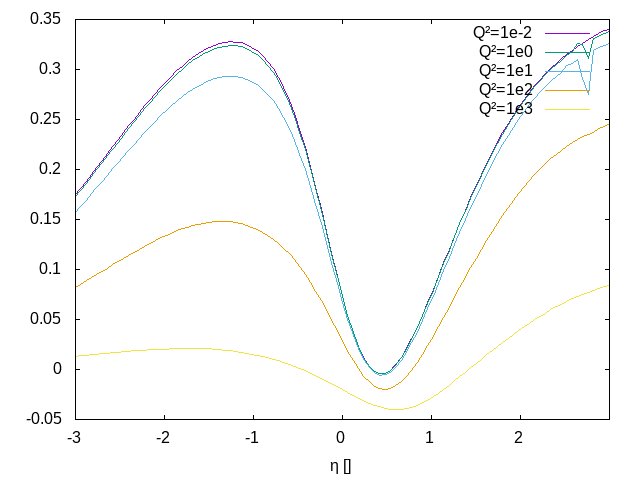
\includegraphics[width=\textwidth]{../../img2/partonic/cg1_VV_F2}
\end{subfigure}%
\begin{subfigure}[t]{.3\textwidth}
	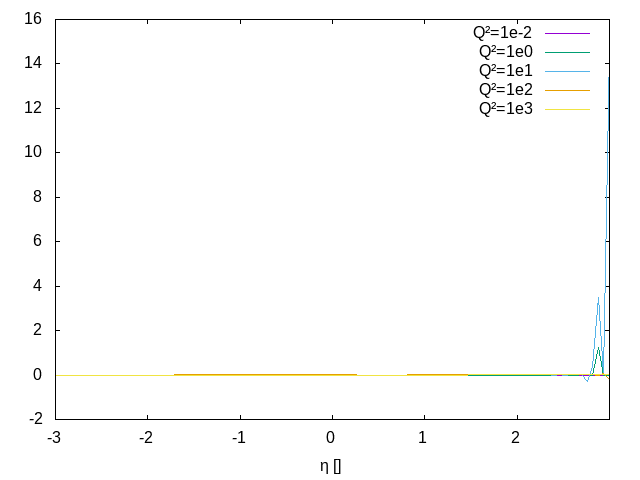
\includegraphics[width=\textwidth]{../../img2/partonic/cg1_VV_FL}
\end{subfigure}%
\begin{subfigure}[t]{.3\textwidth}
	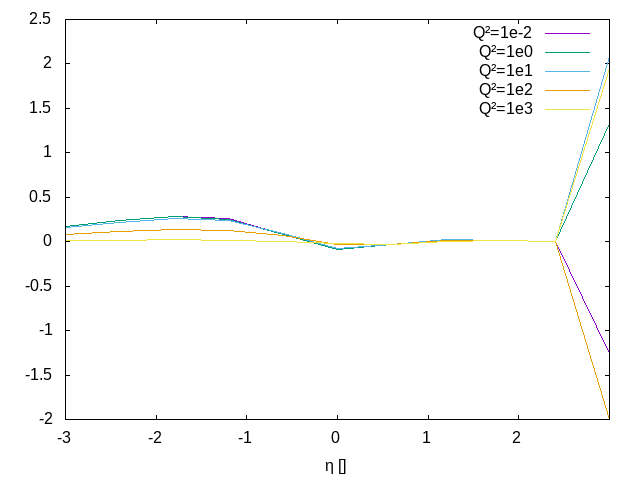
\includegraphics[width=\textwidth]{../../img2/partonic/cg1_VV_x2g1}
\end{subfigure}\\%
\begin{subfigure}[t]{.3\textwidth}
	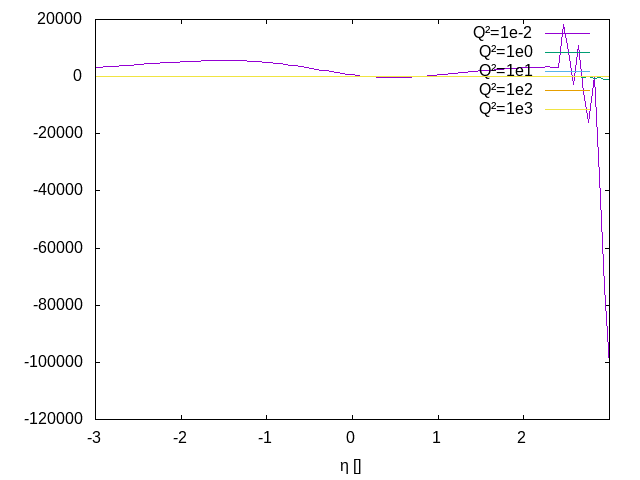
\includegraphics[width=\textwidth]{../../img2/partonic/cg1_AA_F2}
\end{subfigure}%
\begin{subfigure}[t]{.3\textwidth}
	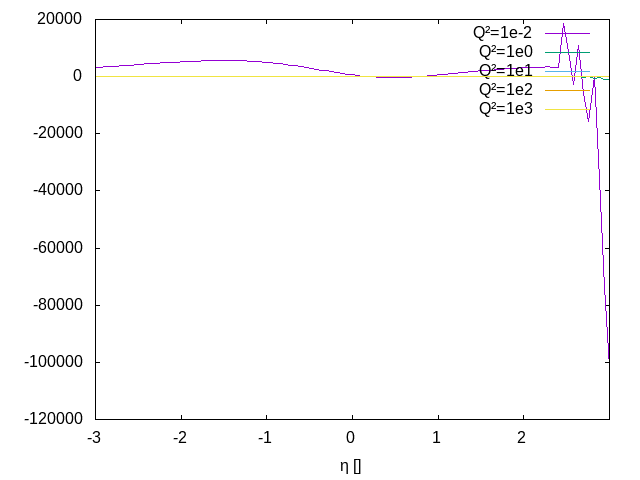
\includegraphics[width=\textwidth]{../../img2/partonic/cg1_AA_FL}
\end{subfigure}%
\begin{subfigure}[t]{.3\textwidth}
	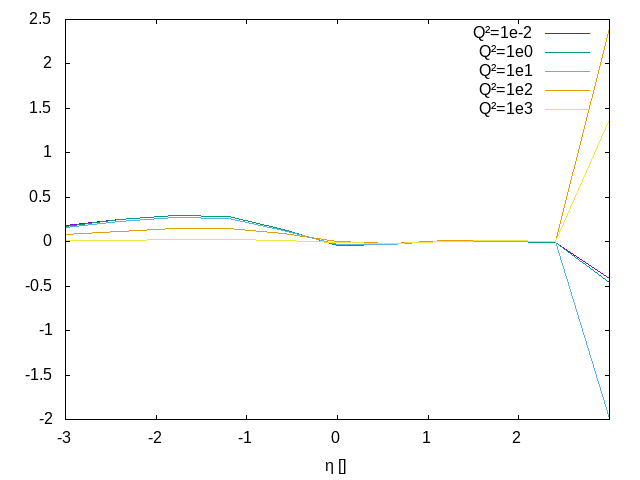
\includegraphics[width=\textwidth]{../../img2/partonic/cg1_AA_x2g1}
\end{subfigure}%
\caption{next-to-leading order scaling functions $c_{k,\Pg}^{(1)}(\eta,\xi)$ plotted as function of $\eta=s/(4m^2)-1$ for different values of $Q^2$ in units of $\si{\GeV^2}$ at $m=\SI{4.75}{\GeV}$ (i.e. different values of $\xi=Q^2/m^2$) }\label{fig:cg1}
\end{figure}
